% Options for packages loaded elsewhere
\PassOptionsToPackage{unicode}{hyperref}
\PassOptionsToPackage{hyphens}{url}
%
\documentclass[
]{article}
\usepackage{amsmath,amssymb}
\usepackage{iftex}
\ifPDFTeX
  \usepackage[T1]{fontenc}
  \usepackage[utf8]{inputenc}
  \usepackage{textcomp} % provide euro and other symbols
\else % if luatex or xetex
  \usepackage{unicode-math} % this also loads fontspec
  \defaultfontfeatures{Scale=MatchLowercase}
  \defaultfontfeatures[\rmfamily]{Ligatures=TeX,Scale=1}
\fi
\usepackage{lmodern}
\ifPDFTeX\else
  % xetex/luatex font selection
\fi
% Use upquote if available, for straight quotes in verbatim environments
\IfFileExists{upquote.sty}{\usepackage{upquote}}{}
\IfFileExists{microtype.sty}{% use microtype if available
  \usepackage[]{microtype}
  \UseMicrotypeSet[protrusion]{basicmath} % disable protrusion for tt fonts
}{}
\makeatletter
\@ifundefined{KOMAClassName}{% if non-KOMA class
  \IfFileExists{parskip.sty}{%
    \usepackage{parskip}
  }{% else
    \setlength{\parindent}{0pt}
    \setlength{\parskip}{6pt plus 2pt minus 1pt}}
}{% if KOMA class
  \KOMAoptions{parskip=half}}
\makeatother
\usepackage{xcolor}
\usepackage[margin=1in]{geometry}
\usepackage{color}
\usepackage{fancyvrb}
\newcommand{\VerbBar}{|}
\newcommand{\VERB}{\Verb[commandchars=\\\{\}]}
\DefineVerbatimEnvironment{Highlighting}{Verbatim}{commandchars=\\\{\}}
% Add ',fontsize=\small' for more characters per line
\usepackage{framed}
\definecolor{shadecolor}{RGB}{248,248,248}
\newenvironment{Shaded}{\begin{snugshade}}{\end{snugshade}}
\newcommand{\AlertTok}[1]{\textcolor[rgb]{0.94,0.16,0.16}{#1}}
\newcommand{\AnnotationTok}[1]{\textcolor[rgb]{0.56,0.35,0.01}{\textbf{\textit{#1}}}}
\newcommand{\AttributeTok}[1]{\textcolor[rgb]{0.13,0.29,0.53}{#1}}
\newcommand{\BaseNTok}[1]{\textcolor[rgb]{0.00,0.00,0.81}{#1}}
\newcommand{\BuiltInTok}[1]{#1}
\newcommand{\CharTok}[1]{\textcolor[rgb]{0.31,0.60,0.02}{#1}}
\newcommand{\CommentTok}[1]{\textcolor[rgb]{0.56,0.35,0.01}{\textit{#1}}}
\newcommand{\CommentVarTok}[1]{\textcolor[rgb]{0.56,0.35,0.01}{\textbf{\textit{#1}}}}
\newcommand{\ConstantTok}[1]{\textcolor[rgb]{0.56,0.35,0.01}{#1}}
\newcommand{\ControlFlowTok}[1]{\textcolor[rgb]{0.13,0.29,0.53}{\textbf{#1}}}
\newcommand{\DataTypeTok}[1]{\textcolor[rgb]{0.13,0.29,0.53}{#1}}
\newcommand{\DecValTok}[1]{\textcolor[rgb]{0.00,0.00,0.81}{#1}}
\newcommand{\DocumentationTok}[1]{\textcolor[rgb]{0.56,0.35,0.01}{\textbf{\textit{#1}}}}
\newcommand{\ErrorTok}[1]{\textcolor[rgb]{0.64,0.00,0.00}{\textbf{#1}}}
\newcommand{\ExtensionTok}[1]{#1}
\newcommand{\FloatTok}[1]{\textcolor[rgb]{0.00,0.00,0.81}{#1}}
\newcommand{\FunctionTok}[1]{\textcolor[rgb]{0.13,0.29,0.53}{\textbf{#1}}}
\newcommand{\ImportTok}[1]{#1}
\newcommand{\InformationTok}[1]{\textcolor[rgb]{0.56,0.35,0.01}{\textbf{\textit{#1}}}}
\newcommand{\KeywordTok}[1]{\textcolor[rgb]{0.13,0.29,0.53}{\textbf{#1}}}
\newcommand{\NormalTok}[1]{#1}
\newcommand{\OperatorTok}[1]{\textcolor[rgb]{0.81,0.36,0.00}{\textbf{#1}}}
\newcommand{\OtherTok}[1]{\textcolor[rgb]{0.56,0.35,0.01}{#1}}
\newcommand{\PreprocessorTok}[1]{\textcolor[rgb]{0.56,0.35,0.01}{\textit{#1}}}
\newcommand{\RegionMarkerTok}[1]{#1}
\newcommand{\SpecialCharTok}[1]{\textcolor[rgb]{0.81,0.36,0.00}{\textbf{#1}}}
\newcommand{\SpecialStringTok}[1]{\textcolor[rgb]{0.31,0.60,0.02}{#1}}
\newcommand{\StringTok}[1]{\textcolor[rgb]{0.31,0.60,0.02}{#1}}
\newcommand{\VariableTok}[1]{\textcolor[rgb]{0.00,0.00,0.00}{#1}}
\newcommand{\VerbatimStringTok}[1]{\textcolor[rgb]{0.31,0.60,0.02}{#1}}
\newcommand{\WarningTok}[1]{\textcolor[rgb]{0.56,0.35,0.01}{\textbf{\textit{#1}}}}
\usepackage{graphicx}
\makeatletter
\def\maxwidth{\ifdim\Gin@nat@width>\linewidth\linewidth\else\Gin@nat@width\fi}
\def\maxheight{\ifdim\Gin@nat@height>\textheight\textheight\else\Gin@nat@height\fi}
\makeatother
% Scale images if necessary, so that they will not overflow the page
% margins by default, and it is still possible to overwrite the defaults
% using explicit options in \includegraphics[width, height, ...]{}
\setkeys{Gin}{width=\maxwidth,height=\maxheight,keepaspectratio}
% Set default figure placement to htbp
\makeatletter
\def\fps@figure{htbp}
\makeatother
\setlength{\emergencystretch}{3em} % prevent overfull lines
\providecommand{\tightlist}{%
  \setlength{\itemsep}{0pt}\setlength{\parskip}{0pt}}
\setcounter{secnumdepth}{-\maxdimen} % remove section numbering
\ifLuaTeX
  \usepackage{selnolig}  % disable illegal ligatures
\fi
\IfFileExists{bookmark.sty}{\usepackage{bookmark}}{\usepackage{hyperref}}
\IfFileExists{xurl.sty}{\usepackage{xurl}}{} % add URL line breaks if available
\urlstyle{same}
\hypersetup{
  pdftitle={Funding Report: Goldberg Gator Engineering Explorers Summer Program 2023},
  pdfauthor={Krista D. Chisholm},
  hidelinks,
  pdfcreator={LaTeX via pandoc}}

\title{Funding Report: Goldberg Gator Engineering Explorers Summer
Program 2023}
\author{Krista D. Chisholm}
\date{2023-10-02}

\begin{document}
\maketitle

{
\setcounter{tocdepth}{2}
\tableofcontents
}
\begin{Shaded}
\begin{Highlighting}[]
\FunctionTok{summary}\NormalTok{(cars)}
\end{Highlighting}
\end{Shaded}

\begin{verbatim}
##      speed           dist       
##  Min.   : 4.0   Min.   :  2.00  
##  1st Qu.:12.0   1st Qu.: 26.00  
##  Median :15.0   Median : 36.00  
##  Mean   :15.4   Mean   : 42.98  
##  3rd Qu.:19.0   3rd Qu.: 56.00  
##  Max.   :25.0   Max.   :120.00
\end{verbatim}

\includegraphics{GGEE_23_Summer_FinalReport_files/figure-latex/pressure-1.pdf}

\hypertarget{summary}{%
\section{Summary}\label{summary}}

The Goldberg Gator Engineering Explorers (GGEE) Summer Program was
designed to provide middle school students with an authentic experience
in programming, engineering design, and computational thinking. The 2023
Summer Program successfully engaged 319 students across 8 school
districts. Students developed computational thinking skills through
design-based challenges using micro:bit micro-controllers.

Schools and Districts partnered with the GGEE program to host programs
and sponsor teachers and materials for the programs at their schools.
There were 20 local teachers that lead summer programs in their area.
Twenty undergraduate engineering students from the University of Florida
and neighboring colleges and universities supported teacher leaders and
served as mentors for students in the program. Both teachers and
undergraduate mentors were trained in program activities to upskill
their abilities in programming, computational thinking, engineering
desgin, and teaching practices. Two grant staff coordinated and ran the
programs.

----DATA

Demographics How students enjoyed the program Growth from beginning to
end

Follow up after-school programs in 5 districts for 12 sessions with
around 200 students participating in the program.

Program costs per student

\textbf{Last year summary} \emph{Students reported they felt challenged
during the program but were rewarded when their code or design worked.
They also mentioned the importance of collaboration with peers to solve
engineering problems, and they enjoyed the mentorship of the college
students working with the program. The longitudinal effects of the
summer program on grades in math and science and students' enrollment in
higher-level courses will be tracked by the research study for the
program. All districts provided in-kind donations to the camp, and many
school districts have plans to host or expand the programs for next
year. Some schools have asked about follow-up programming, including
afterschool programming to continue student engagement. The cost per
student for the program was \$996, including all costs for program
development (three months), camp costs (two months), and post-assessment
of the program. The cost per student for future camps should be less
owing to development costs built into the program's first year.}

\hypertarget{introduction}{%
\section{Introduction}\label{introduction}}

\hypertarget{background}{%
\subsection{Background}\label{background}}

The Goldberg Gator Engineering Explorers Summer Program was initiated by
a generous donor, Arnold Goldberg, to the University of Florida
Foundation. He envisioned a free summer program for underrepresented
minority middle school students. The program would allow students to
experience computer science and have opportunities to learn to not only
program but build skills in computational thinking, problem solving, and
engineering design. The vision was brought to life by the EQuIPD grant
at the University of Florida. Their team developed introductory and
advanced-level summer programs and have worked with schools and
districts to host the programs across the state of Florida.

The Goldberg Gator Engineering Explorers Program was designed to
introduce middle school-aged students to programming and computer
science. The program begins with students learning the base elements of
coding through small activities that engage them in applying concepts
such as strings, conditional statements, loops, and variables. They use
these concepts and the micro:bit to develop a simple game and to also
collect and analyze light intensity data to study the relationship of
light intensity and distance. The program then has students working on
two scaling design challenges with partners and teams. The first is a
creative engineering design challenge where they create a micro:bit pet
for a partner. Then second is a technical design challenge where teams
create a solution to a local problem - traffic lights for emergency
service vehicles, environmental sensors for a farmer, and an indicator
for new drivers.

After the pilot program during the summer of 2022,

Provide a brief overview of the middle school summer program, including
its purpose and objectives. Highlight why the program was initiated and
its importance in the district.

\hypertarget{purpose-of-the-report}{%
\subsection{Purpose of the Report}\label{purpose-of-the-report}}

\emph{Explain the purpose of this final report and what the reader can
expect to find within it.}

\hypertarget{district-recruitment}{%
\section{District Recruitment}\label{district-recruitment}}

\hypertarget{recruitment-strategies}{%
\subsection{Recruitment Strategies}\label{recruitment-strategies}}

\emph{Detail the strategies used to recruit students for the program.
Discuss any partnerships or collaborations that helped with recruitment
efforts.}

\hypertarget{participant-selection-criteria}{%
\subsection{Participant Selection
Criteria}\label{participant-selection-criteria}}

\emph{Explain the criteria used to select participants for the program.
This could include grade level, academic standing, or other factors.}

School Recruitment

\hypertarget{summer-programs}{%
\section{Summer Programs}\label{summer-programs}}

\hypertarget{vs.-2023}{%
\subsection{2022 vs.~2023}\label{vs.-2023}}

\begin{figure}
\centering
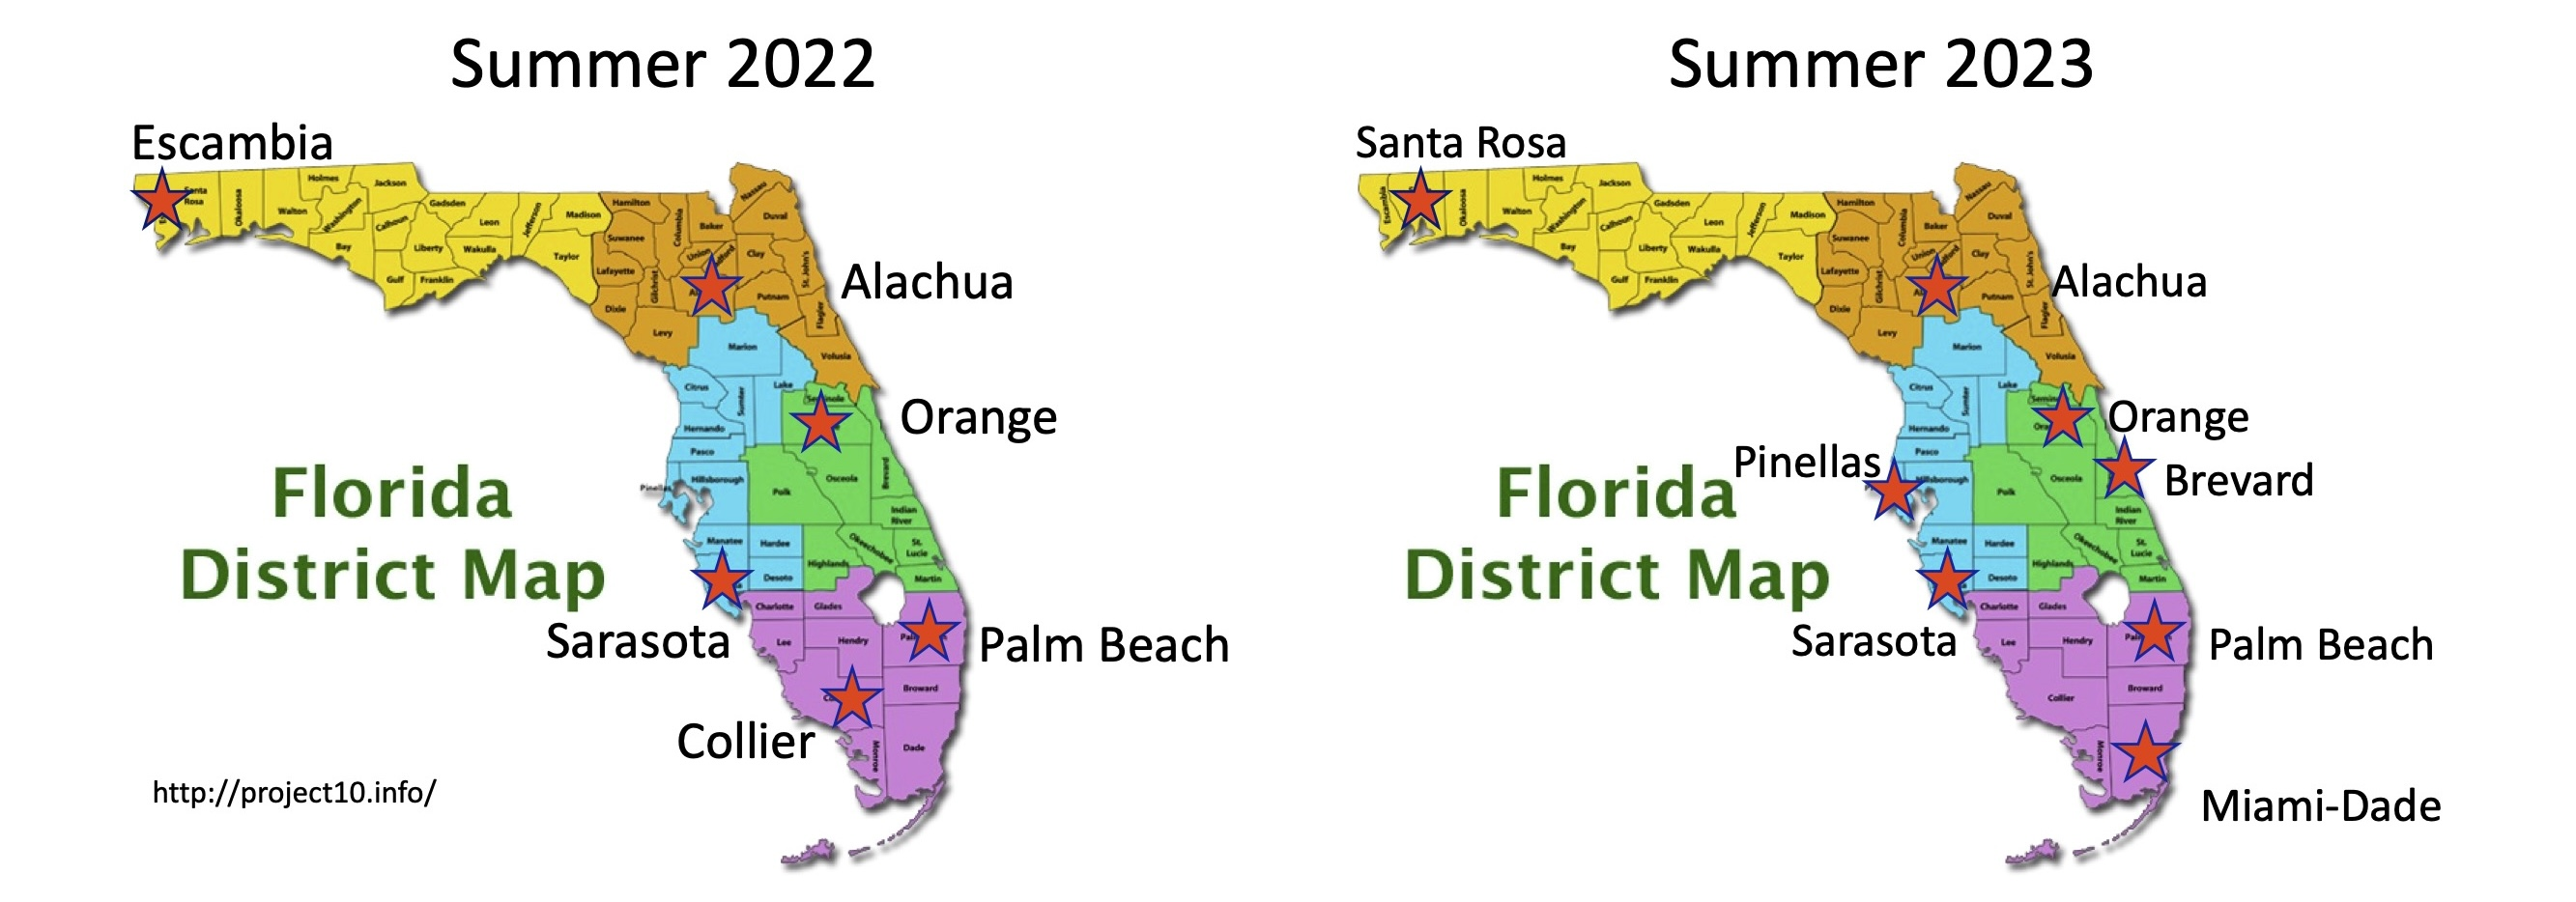
\includegraphics{/Users/kristadulany/Documents/GitHub/GGEESummer23/Graphs/GGEE_23_FL District Map.jpg}
\caption{\emph{2023 Summer Program Calendar}}
\end{figure}

\hypertarget{program-calendar}{%
\subsection{Program Calendar}\label{program-calendar}}

\emph{Provide an overview of the program's calendar, including the
duration of the program, daily schedules, and key activities.}

There were X many programs in each district

\begin{figure}
\centering
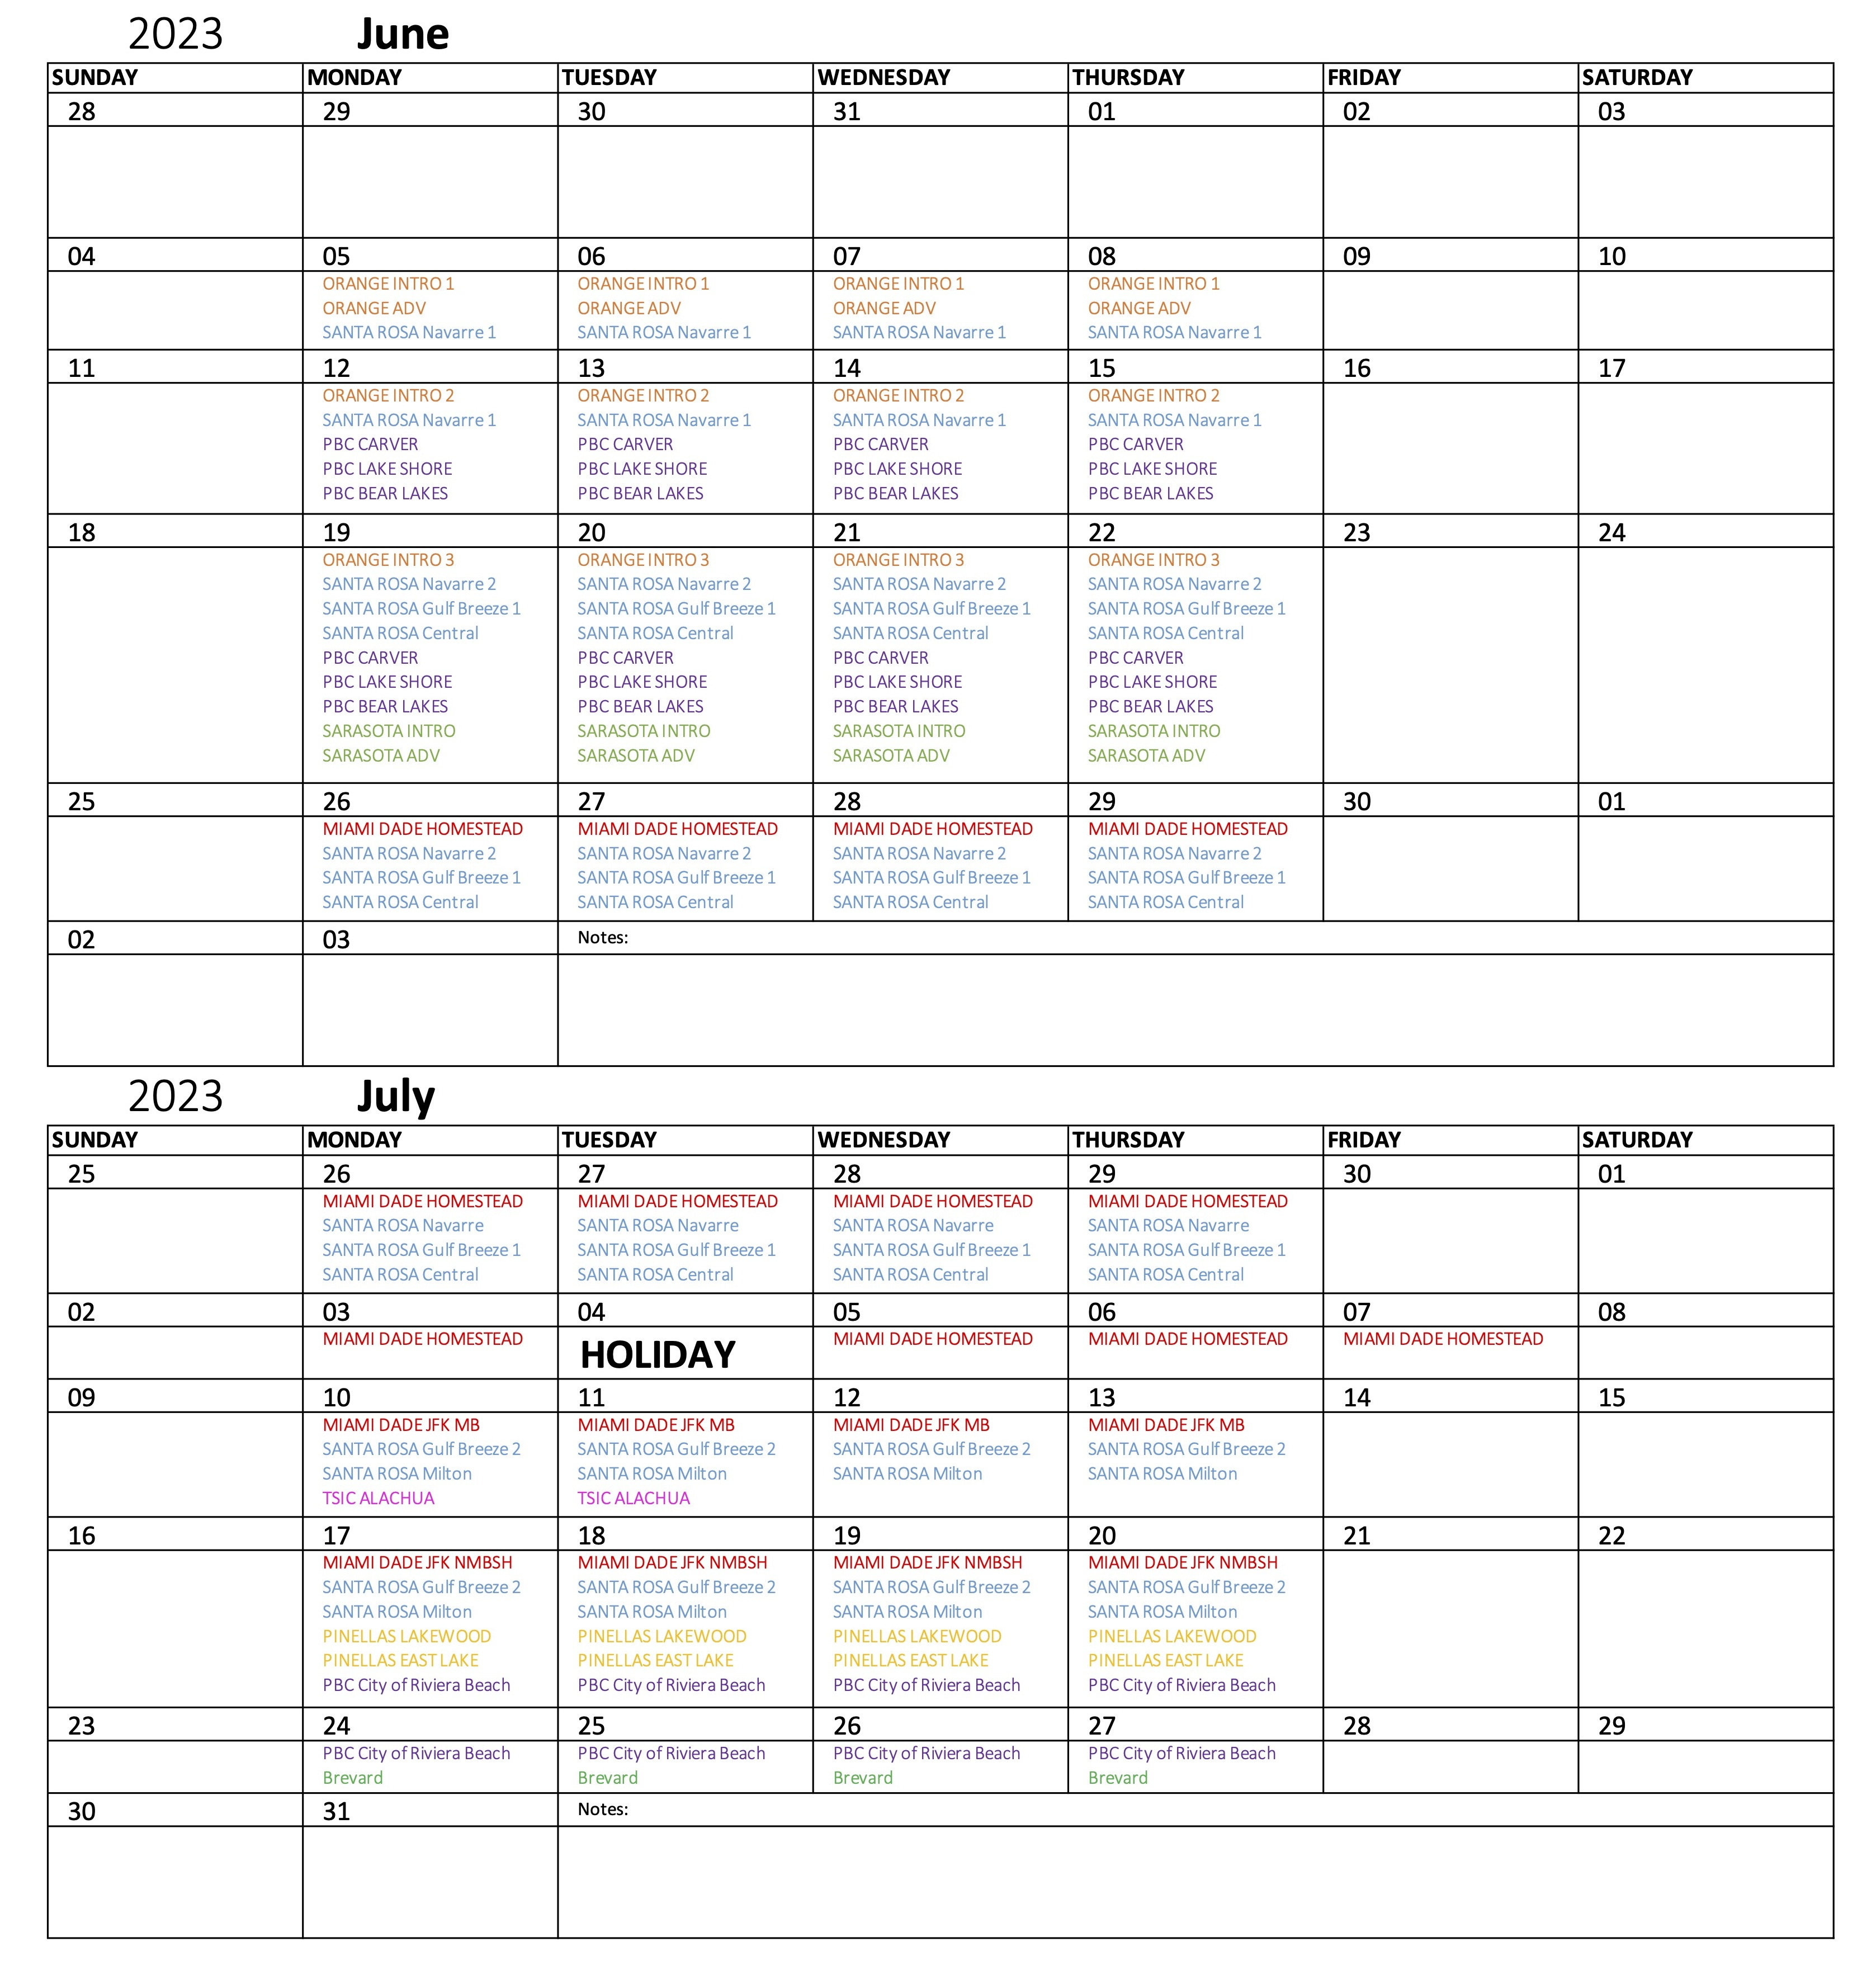
\includegraphics{/Users/kristadulany/Documents/GitHub/GGEESummer23/Graphs/GGEE_23_Calendar.jpg}
\caption{\emph{2023 Goldberg Gator Engineering Explorers Summer Program
Calendar}}
\end{figure}

\hypertarget{program-layouts}{%
\subsection{Program Layouts}\label{program-layouts}}

\hypertarget{day-programs}{%
\subsubsection{4-Day Programs}\label{day-programs}}

\hypertarget{day-programs-1}{%
\subsubsection{8-Day Programs}\label{day-programs-1}}

\hypertarget{youth-compliance}{%
\section{Youth Compliance}\label{youth-compliance}}

\hypertarget{waivers-and-research-consent}{%
\subsection{Waivers and Research
Consent}\label{waivers-and-research-consent}}

\hypertarget{storage-of-student-information}{%
\subsection{Storage of Student
Information}\label{storage-of-student-information}}

\hypertarget{institutional-review-board}{%
\subsection{Institutional Review
Board}\label{institutional-review-board}}

\hypertarget{program-numbers}{%
\section{Program Numbers}\label{program-numbers}}

\hypertarget{enrollment-statistics}{%
\subsection{Enrollment Statistics}\label{enrollment-statistics}}

\emph{Present enrollment data, including the number of students who
initially registered, and any changes over the course of the program.}

Programs were able to host up to 25 students in each of their program
sessions. Registrations were closed and students were placed on wait
lists in the case of cancellations by student parents. Programs had on
average X number of students enroll. Wait lists ranged from 5 - 80
students in some districts.

Bar Graph Comparison - Total Number of Registered Students - stacked bar
graph - registered vs waitlist

\textbf{GRAPH by Session - stacked graph - regsitered vs waitlist}

Need for more programs in Santa Rosa County District Schools

\hypertarget{attendance-records}{%
\subsection{Attendance Records}\label{attendance-records}}

\emph{Share attendance records to illustrate the level of student
engagement and participation throughout the program.}

Actual attendance with the programs were less than initial
registrations. Students became ill, were unable to attend the first days
of the program or parents made new plans for their families.

\textbf{GRAPH Attendance Numbers by School}

\begin{figure}
\centering
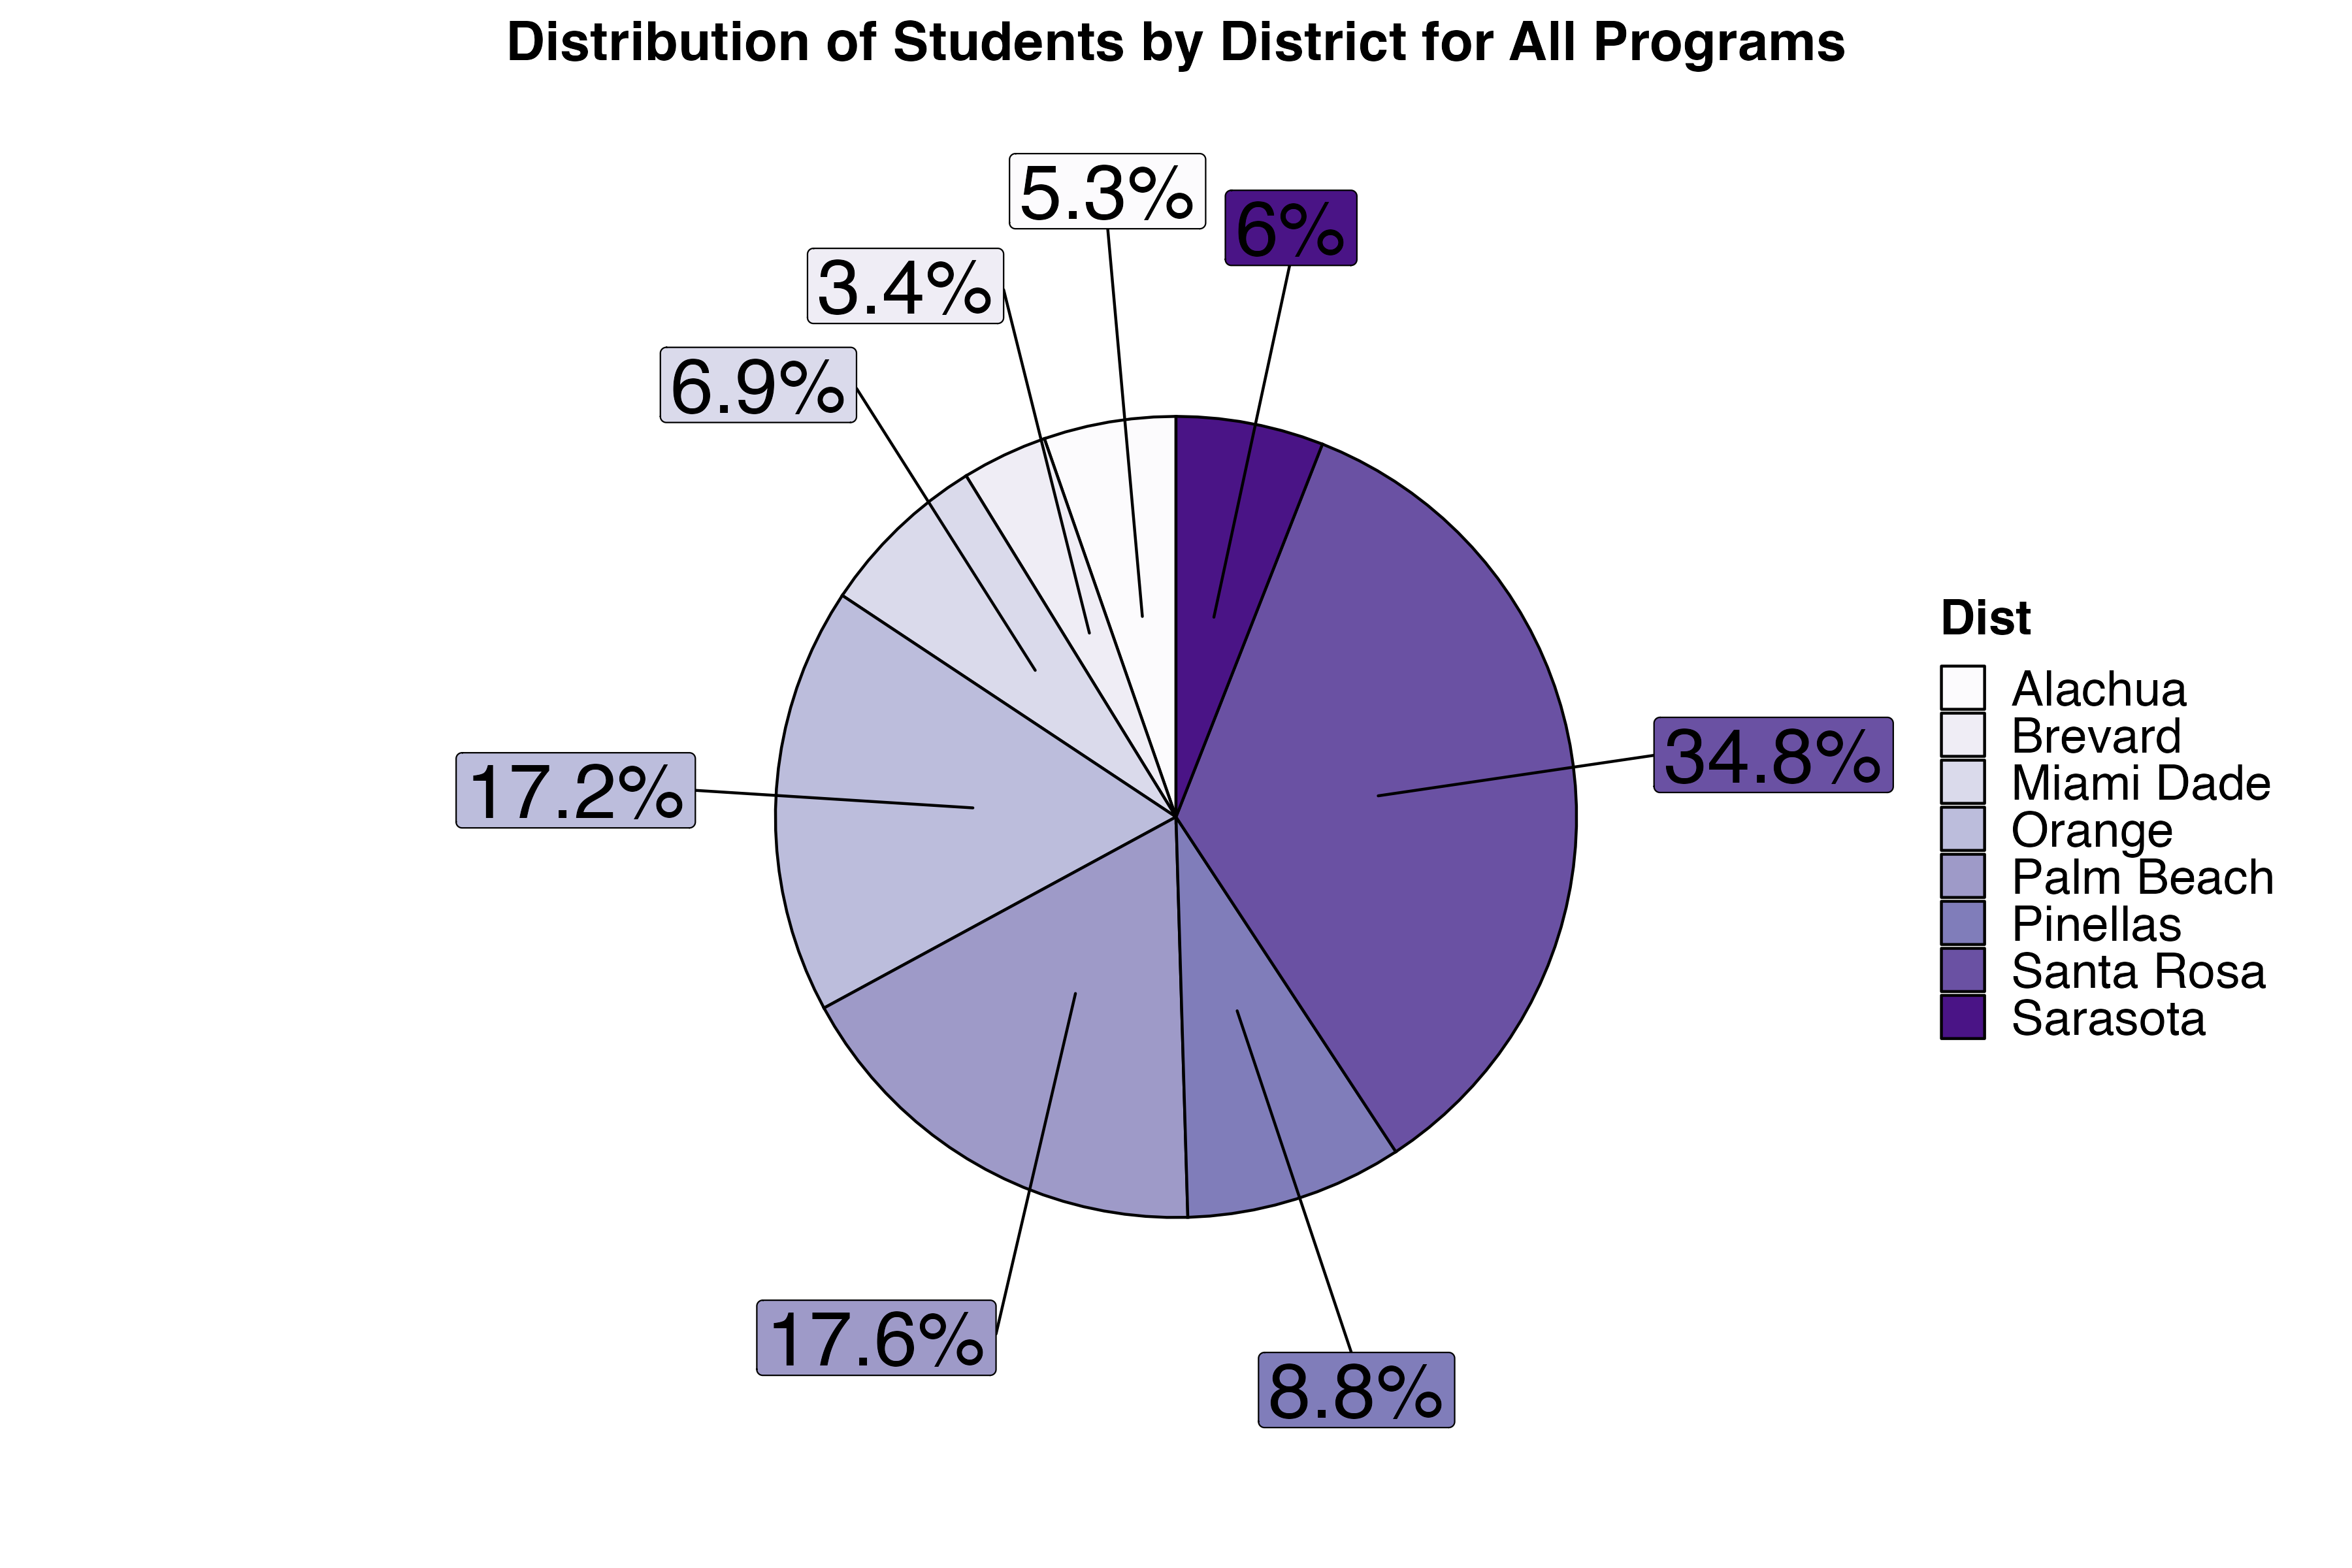
\includegraphics{/Users/kristadulany/Documents/GitHub/GGEESummer23/Graphs/All Camps/GGEE_23_Summer_Pie_ALL.png}
\caption{How many of the 319 students participating in the GGEE Summer
Programs were from each Florida school district.}
\end{figure}

\hypertarget{student-demographics}{%
\section{Student Demographics}\label{student-demographics}}

\hypertarget{age}{%
\subsection{Age}\label{age}}

\emph{Include demographic information such as age, gender, ethnicity,
and socioeconomic background of the participating students.}

Demographics were collected on students participating in the research
study.

\begin{figure}
\centering
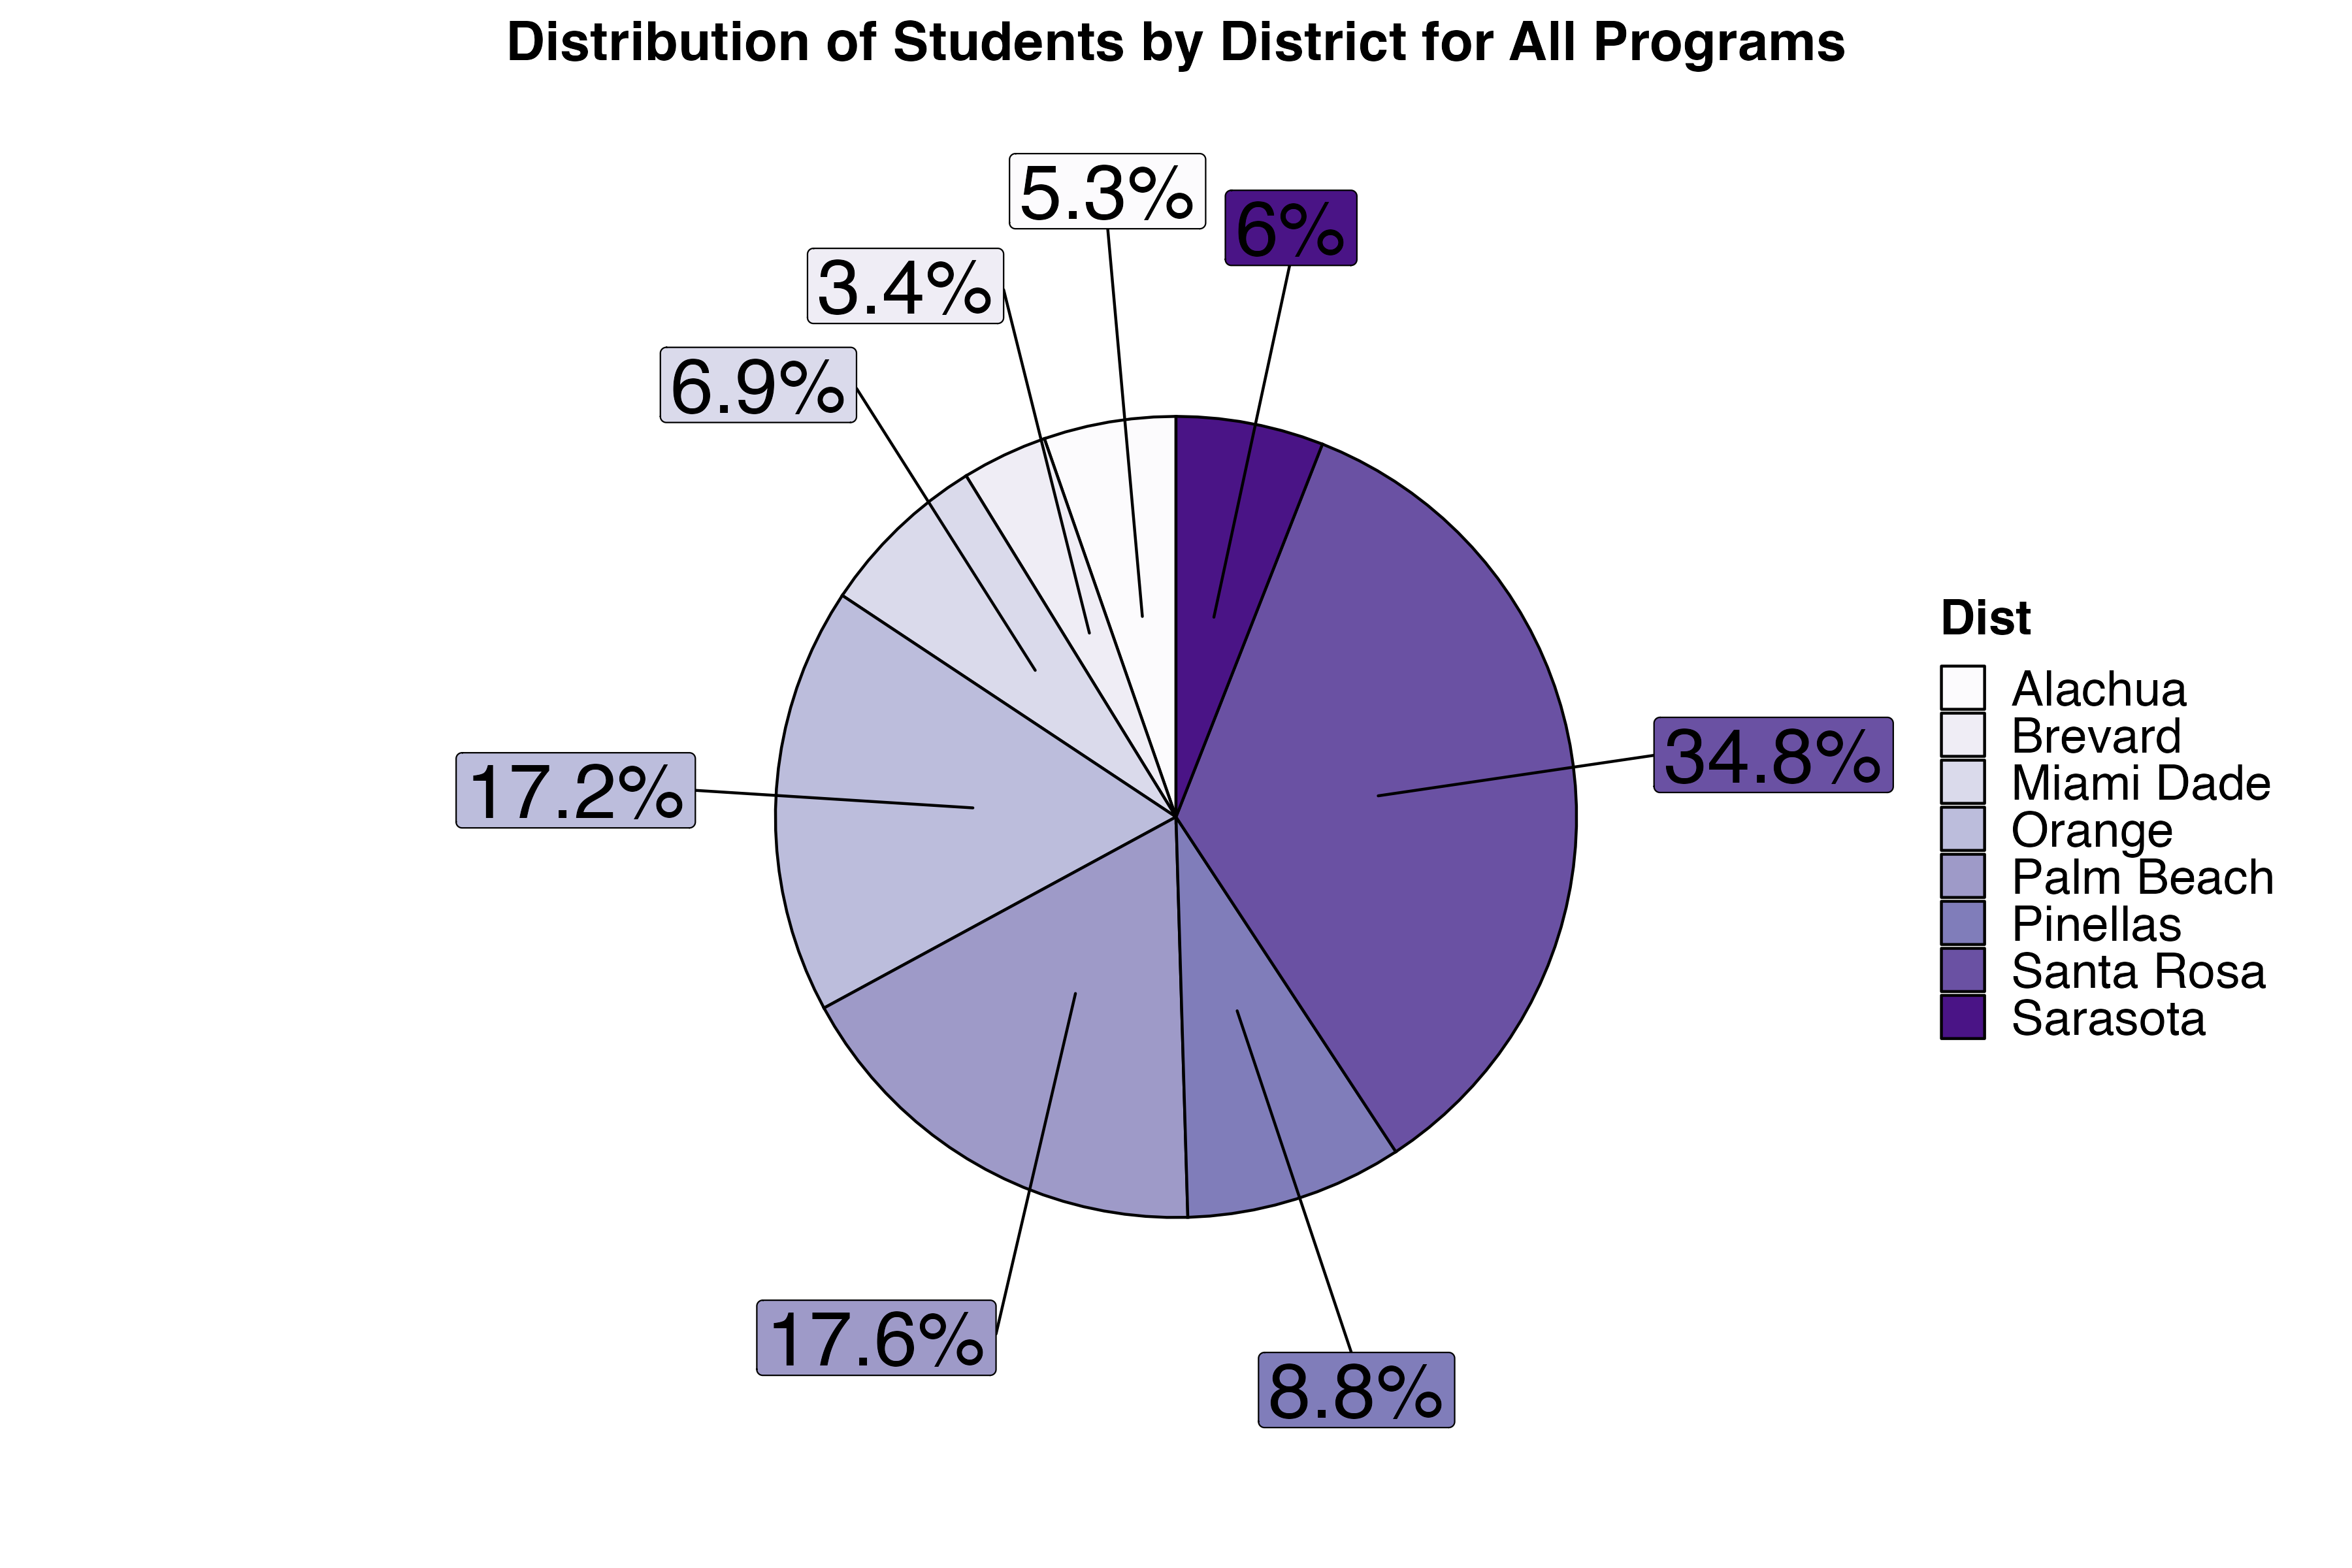
\includegraphics{/Users/kristadulany/Documents/GitHub/GGEESummer23/Graphs/All Camps/GGEE_23_Summer_Pie_ALL.png}
\caption{How many of the 319 students participating in the GGEE Summer
Programs were from each Florida school district.}
\end{figure}

\hypertarget{gender}{%
\subsection{Gender}\label{gender}}

\hypertarget{race-and-ethnicity}{%
\subsection{Race and Ethnicity}\label{race-and-ethnicity}}

\hypertarget{section}{%
\subsection{}\label{section}}

\hypertarget{pre-survey-responses}{%
\section{Pre-Survey Responses}\label{pre-survey-responses}}

\hypertarget{summary-of-pre-program-survey-results}{%
\subsection{Summary of Pre-Program Survey
Results}\label{summary-of-pre-program-survey-results}}

Summarize the responses from the pre-program survey, highlighting key
findings and insights.

\hypertarget{survey-responses}{%
\section{Survey Responses}\label{survey-responses}}

\hypertarget{analysis-of-ongoing-survey-data-if-conducted-during-the-program}{%
\subsection{Analysis of Ongoing Survey Data (if conducted during the
program)}\label{analysis-of-ongoing-survey-data-if-conducted-during-the-program}}

If you conducted surveys during the program, analyze the responses and
share any noteworthy trends or changes over time.

\hypertarget{student-interviews}{%
\section{Student Interviews}\label{student-interviews}}

\hypertarget{highlights-from-student-interviews}{%
\subsection{Highlights from Student
Interviews}\label{highlights-from-student-interviews}}

Share significant insights and quotes gathered from student interviews,
emphasizing their experiences and perspectives.

\hypertarget{final-program-survey-responses}{%
\section{Final Program Survey
Responses}\label{final-program-survey-responses}}

\hypertarget{summary-of-post-program-survey-results}{%
\subsection{Summary of Post-Program Survey
Results}\label{summary-of-post-program-survey-results}}

Present the results of the post-program survey, emphasizing any changes
in student responses compared to the pre-program survey.

\hypertarget{program-outcomes}{%
\section{Program Outcomes}\label{program-outcomes}}

\hypertarget{assessment-of-program-objectives-and-goals}{%
\subsection{Assessment of Program Objectives and
Goals}\label{assessment-of-program-objectives-and-goals}}

Evaluate whether the program met its objectives and goals as outlined in
the introduction.

\hypertarget{challenges-and-lessons-learned}{%
\section{Challenges and Lessons
Learned}\label{challenges-and-lessons-learned}}

\hypertarget{identification-of-challenges-faced}{%
\subsection{Identification of Challenges
Faced}\label{identification-of-challenges-faced}}

Discuss any challenges encountered during the program's implementation.

\hypertarget{lessons-learned-and-adaptations-made}{%
\subsection{Lessons Learned and Adaptations
Made}\label{lessons-learned-and-adaptations-made}}

Share lessons learned from the program's challenges and any adjustments
or improvements made as a result.

\hypertarget{recommendations}{%
\section{Recommendations}\label{recommendations}}

\hypertarget{suggestions-for-program-improvement}{%
\subsection{Suggestions for Program
Improvement}\label{suggestions-for-program-improvement}}

\emph{Provide recommendations for improving the program in future
iterations, based on the insights gained.}

\begin{itemize}
\tightlist
\item
  Updating compliance forms with more clear langaue for parent and the
  research study
\item
  Make submitting paperwork a part of the registration process. Did this
  with the 2023-2024 After-School programs and it has made everything so
  much easier to process and collect rather than a 2-step process
\item
  Creating contract-like documents to denote needs, requirments, and
  expectations from the schools and what is provided from the GGEE
  program at UF
\item
  Starting Recruitment in November
\item
  ensuring districts cover technology to continue to use in after-school
  programs or integrate into classroom projects
\item
  revise research study to expand to get more teacher and UF
  undergraduate mentor insight in the program
\end{itemize}

\hypertarget{future-directions}{%
\subsection{Future Directions}\label{future-directions}}

\emph{Suggest potential directions for the program's growth or
expansion.}

\hypertarget{conclusion}{%
\section{Conclusion}\label{conclusion}}

\hypertarget{recap-of-programs-successes}{%
\subsection{Recap of Program's
Successes}\label{recap-of-programs-successes}}

Summarize the program's achievements and positive outcomes.

\hypertarget{reiteration-of-impact-on-students}{%
\subsection{Reiteration of Impact on
Students}\label{reiteration-of-impact-on-students}}

Emphasize how the program benefited the participating students and the
broader school community.

\hypertarget{appendices}{%
\section{Appendices}\label{appendices}}

Include any supplementary materials, such as additional data charts and
graphs, the complete survey questions, and interview transcripts.

Please adapt this template to your specific program and add more details
and content as needed to create a comprehensive final report for your
middle school summer program.

\end{document}
